\section{Overall system description}
A simplified class diagram describing the essentials of the system is shown in
figure \ref{fig:impl:sys:uml_complete}. The individual parts are described in
detail in the following sections of this chapter. In this section, the overall
system, flow of data, and external API is described.

It is important to note that, as mentioned, this implementation is a ``proof of
concept'' and only implements a subset of the ``Tainting Dependencies''
method developed and explained in section \ref{chapter:translation}. 

\newpage

\begin{figure}[!htp]
\begin{center}
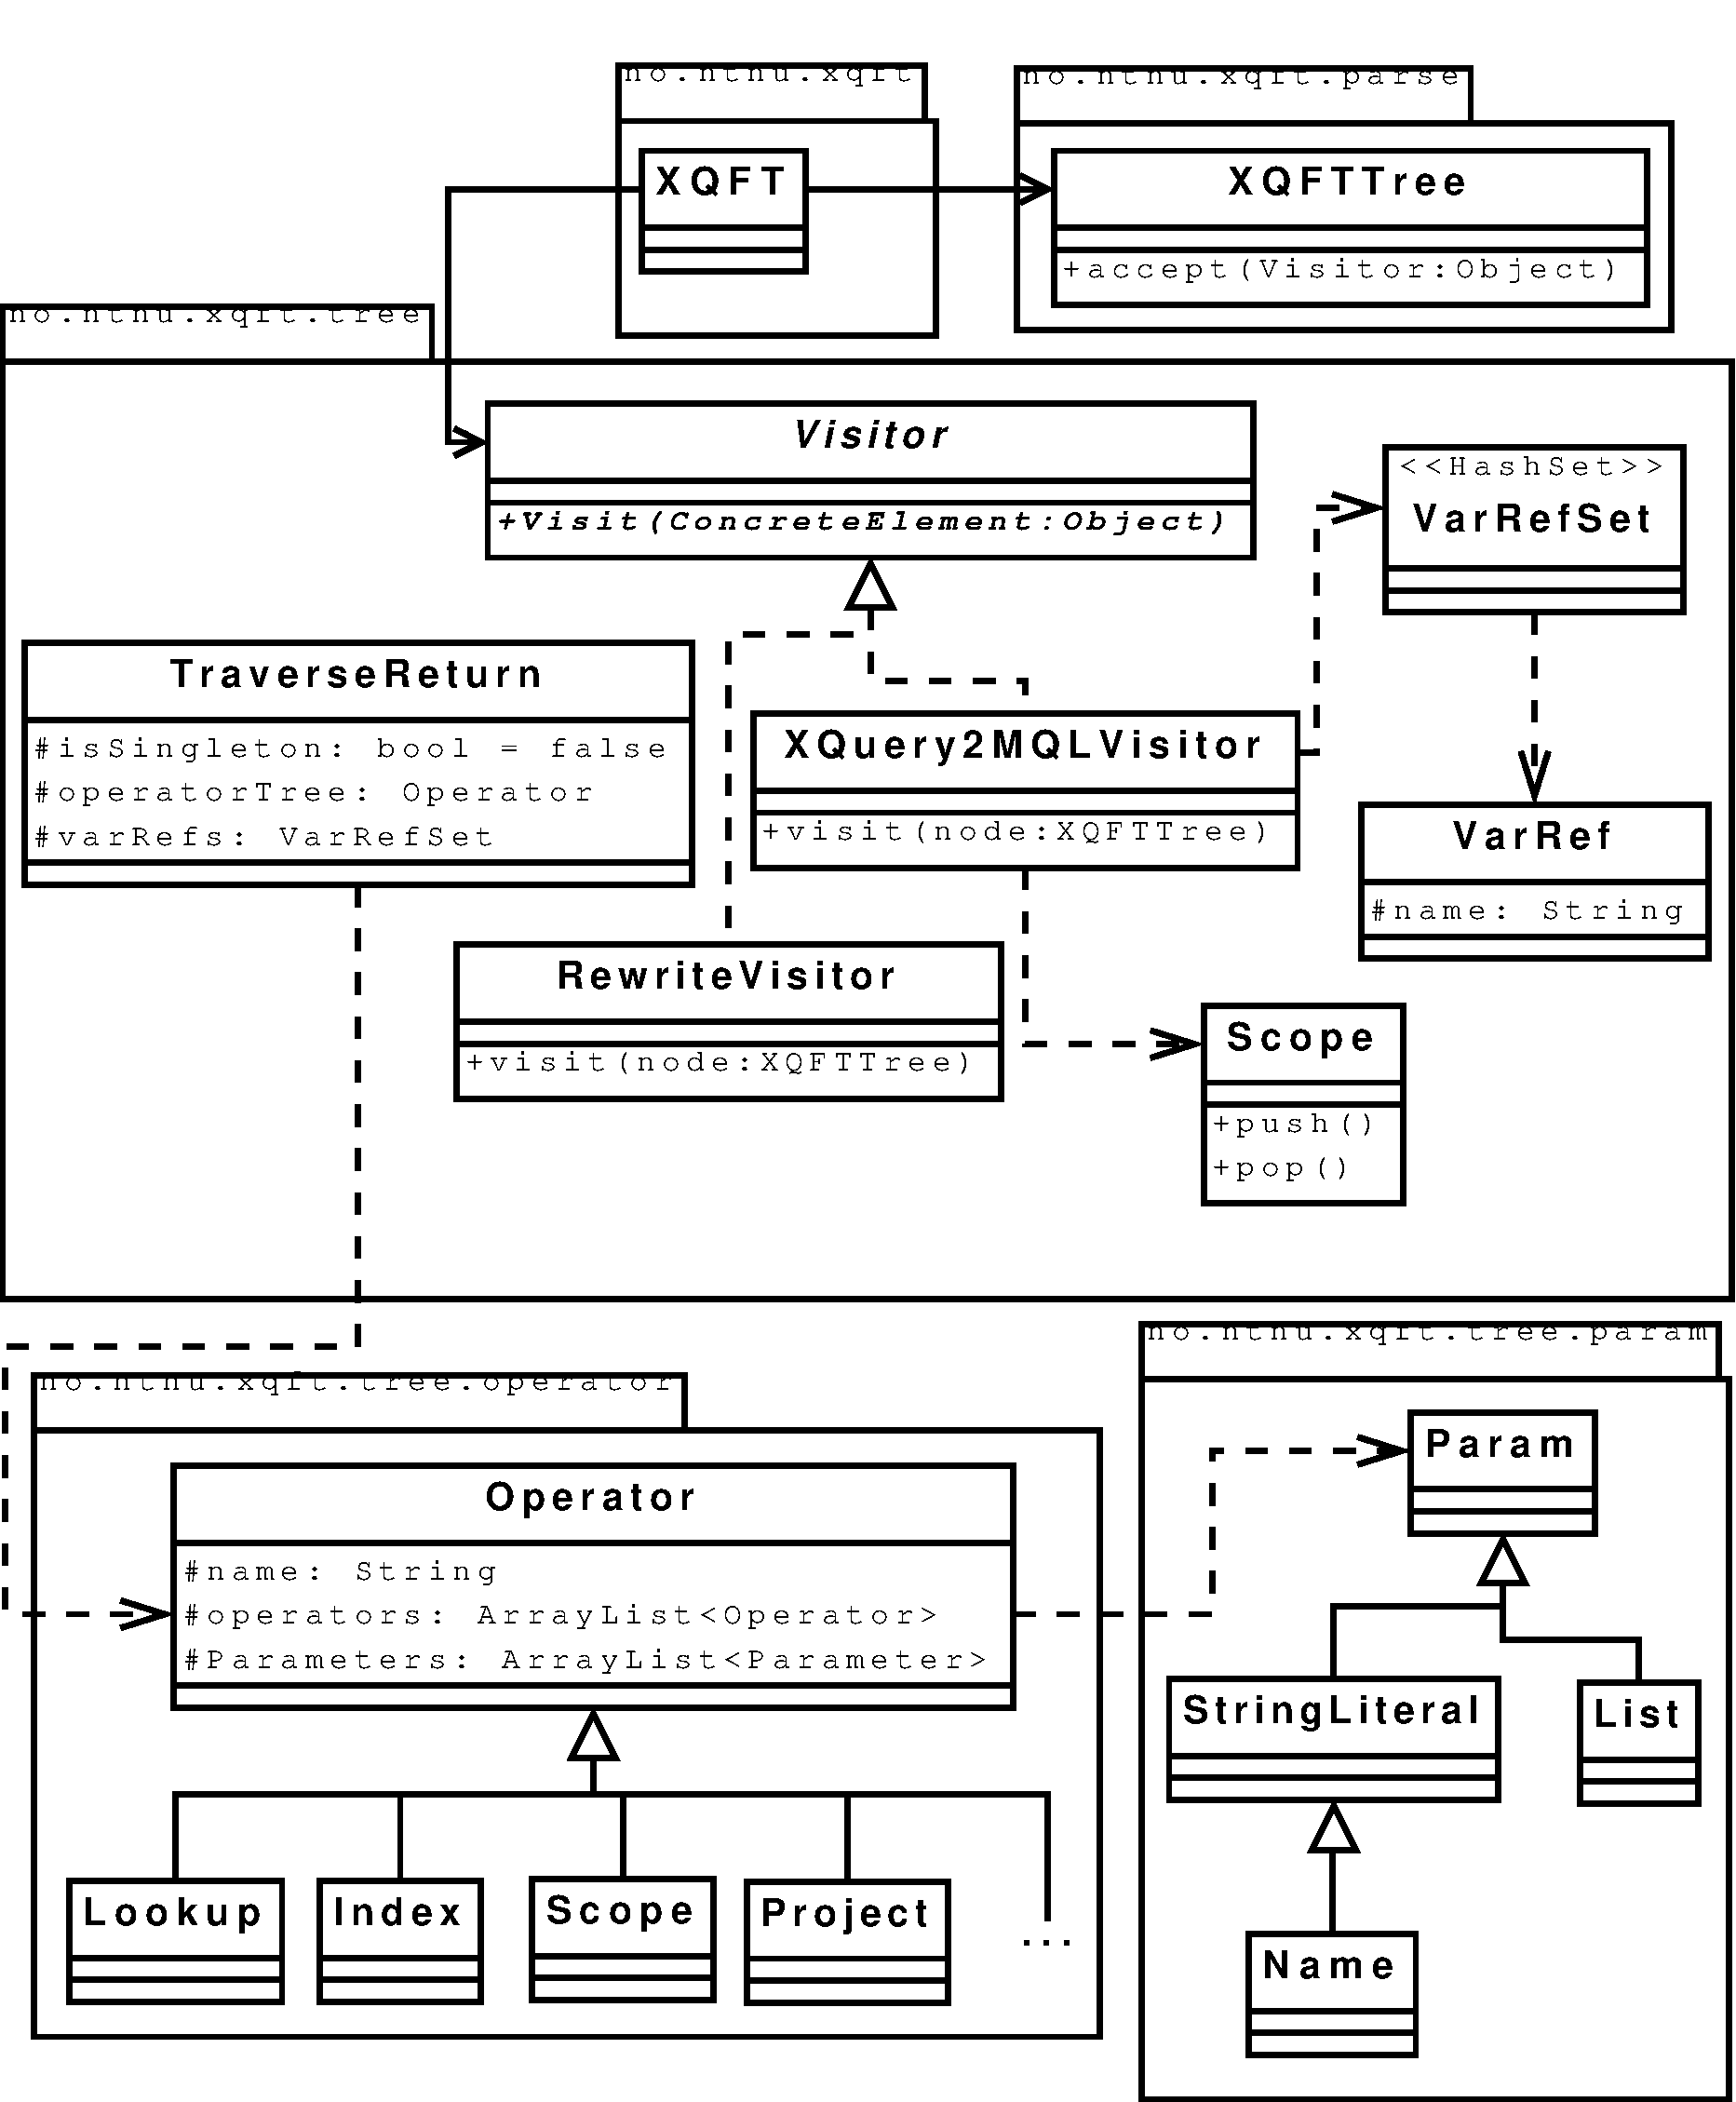
\includegraphics[scale=0.45]{diagrams/complete_uml}
  \caption{Simplified UML for complete implementation}
  \label{fig:impl:sys:uml_complete}
\end{center}
\end{figure}

\subsection{Data flow}
Figure \ref{fig:impl:sys:mql_dataflow} illustrates the flow of data when
translating a XQuery query into a MQL query (see section \ref{sect:method:mql}
on page \pageref{sect:method:mql} for a description of MQL). 

\begin{figure}[!htp]
\begin{center}
  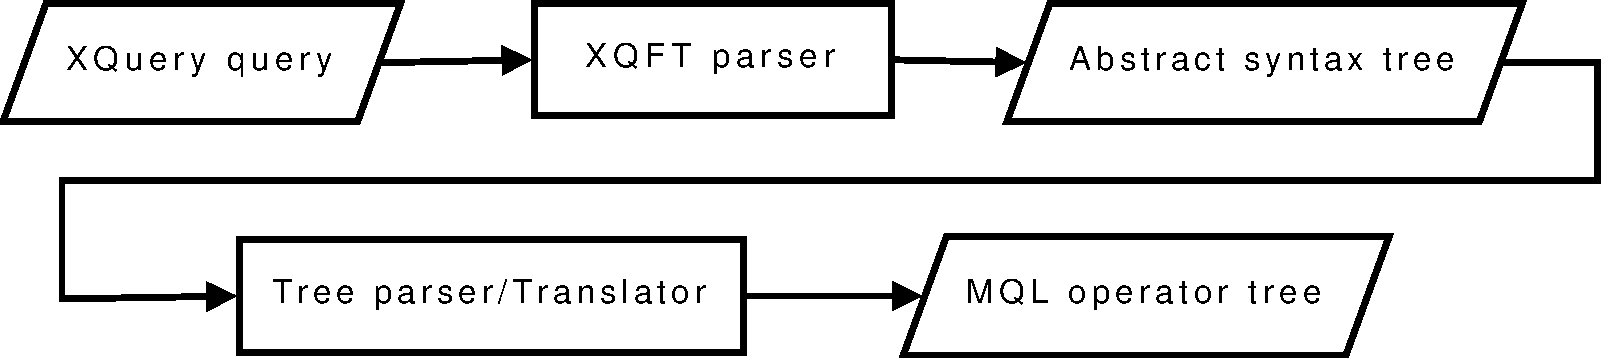
\includegraphics[scale=0.5]{diagrams/mql_dataflow}
  \caption{Data flow for XQuery parsing and translation to MQL}
  \label{fig:impl:sys:mql_dataflow}
\end{center}
\end{figure}

\subsection{Visible external API}
The API available to programmers is defined in a trivial manner in the
\texttt{no.ntnu.xqft.XQFT} class. This class can also be executed as a
standalone application (see next subsection). Figure
\ref{fig:impl:sys:xqft_extapi_uml} describes the \texttt{no.ntnu.xqft.XQFT}
class.

\begin{figure}[!htp]
\begin{center}
  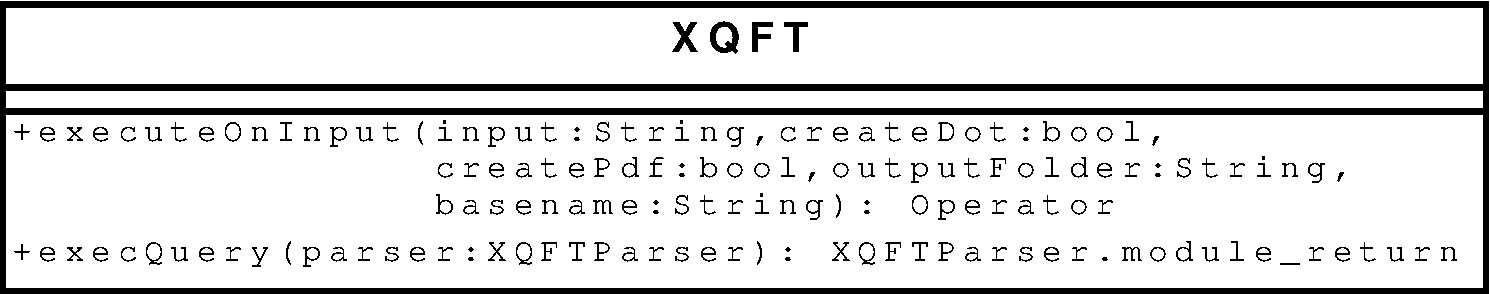
\includegraphics[scale=0.5]{diagrams/xqft_extapi_uml}
  \caption{External API for the XQuery to MQL translator}
  \label{fig:impl:sys:xqft_extapi_uml}
\end{center}
\end{figure}

As can be seen, two methods are primarily available. Out of these two,
\texttt{executeOnInput()} is the most complex, but also the most flexible. A
typical usage scenario for an external user could be as follows:

\begin{Verbatim}
XQFT xqft = new XQFT();
Operator mqlTree = xqft.executeOnInput(
                       "for $i in (1,2,3) return $i", 
                       false, false, null, null
                   );
\end{Verbatim}

The \texttt{mqlTree} would now be a reference to a complete MQL operator tree,
provided that no errors occured during the parse process or the translation
process.

\subsection{Command line interface}
\label{sect:impl:system:cli}
The command line interface is available by executing the
\texttt{no.ntnu.xqft.XQFT} class as a main class, as mentioned in the previous
section. The command line interface uses the Args
Engine\footnote{http://www.adarshr.com/papers/args} for the sake of simplicity
to parse options/switches on the command line. 

The command line usage is as follows:

\begin{Verbatim}
java no.ntnu.xqft.XQFT [-p] [-t] [-o <path>] file1 file2 ... fileN
\end{Verbatim}

It is also possible to specify queries in the form of strings enclosed in
double quotes, or any mix of strings and filenames. The switches are:
\begin{itemize}
  \item -t : output a DOT tree (requires graphviz)
  \item -p : output a PDF syntax tree (requires graphviz)
  \item -o <path> : stores generated PDF/DOT files in the given folder, 
  otherwise in the current folder (simply ./)
\end{itemize}

See appendix \ref{appendix:installation} for more information about installation and
dependencies.
